\documentclass{article} % For LaTeX2e
\usepackage{nips13submit_e,times}
\usepackage{hyperref}
\usepackage{url}
\usepackage{amsmath}
\usepackage{amsfonts}
\usepackage{graphicx}
%\documentstyle[nips13submit_09,times,art10]{article} % For LaTeX 2.09


\title{AM207 Final Project Proposal: Modelling Civil Conflict and Refugee Relief Aid in Uganda}


\author{
Peter J. Bull\\
Institute for Applied Computer Science\\
Harvard University\\
Cambridge, Massachusetts \\
\texttt{bull@fas.harvard.edu} \\
\and
\textbf{Isaac M.~Slavitt}\\
Institute for Applied Computational Science\\
Harvard University\\
Cambridge, Massachusetts\\
\texttt{slavitt@fas.harvard.edu} \\
}

% The \author macro works with any number of authors. There are two commands
% used to separate the names and addresses of multiple authors: \And and \AND.
%
% Using \And between authors leaves it to \LaTeX{} to determine where to break
% the lines. Using \AND forces a linebreak at that point. So, if \LaTeX{}
% puts 3 of 4 authors names on the first line, and the last on the second
% line, try using \AND instead of \And before the third author name.

\newcommand{\fix}{\marginpar{FIX}}
\newcommand{\new}{\marginpar{NEW}}

\nipsfinalcopy % Uncomment for camera-ready version

\begin{document}


\maketitle

\begin{abstract}
Using stochastic modeling techniques learned in AM207, we aim to model civil conflict in Uganda and
optimize the limited relief aid that can be provided in these scenarios. The goal is two-fold: first, 
to simulate civil conflict events given historical data about these events. This could have the benfits
of predict future incidents and modelling the spread of violence during larger-scale civil conflicts. \\
\\
The second goal is to optimize the distribution of limited aid resources to refugees from these crises. Using
features about the geography, demographics and infrastructure of Uganda, we can attempt to find optimal locations
to deliver aid so that the greatest number of refugees from these crises can be served. We will approach this
complex optimization task using stochastic methods from the course.
\end{abstract}

\section{The Data}

The data comes from ACLED (Armed Conflict Location and Event Data Project) [1], which is a dataset with locations, dates, fatalities, motivation, actors involved, and other information about civil conflicts in Africa. Their collection of data on Uganda covers 1997-2013, and they have a real-time tracker of events reported in 2014. This new data from 2014 could be used as a test set for our modeled simulations of violence. The need for an understanding of these patterns of conflict is clear, as ACLED notes:
\begin{quote}
This dataset codes the dates and locations of all reported political violence events in over 50 developing countries. Political violence includes events that occur within civil wars or periods of instability. Although civil war occurrence is decreasing across African countries, new forms of political violence are becoming more common.  [1]
\end{quote}
Given that ACLED has collected data for civil conflict across many developing nations, I hope that the models built for this project can be tested, adapted, and applied to geographic areas outside of Uganda.

For Uganda, the dataset contains around 4500 observations of civil violence. Each observation includes the data, location, an quantified estimate for how precise these measures are, a number of fatalities for the event, and the actors involved.w

\section{Modeling Civil Conflict Events}

\begin{figure}
  \centering
  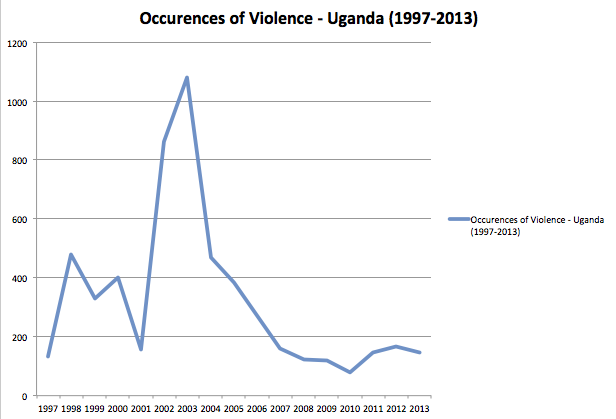
\includegraphics[width=0.8\textwidth]{PerYear.png}
  \caption{Civil conflict per year in Uganda 1997-2013. [2]}
  \label{fig:shells}
\end{figure}

\subsection{Bayesian Poisson Regression}

We will use a bayesian monte-carlo model to simulate drawing samples (civil conflict events) from their underlying distribution. After creating a grid for the country, we will assume that for a given square $i,j$ a civil conflict event:

\begin{align}
Y_{i,j} \sim \text{Poi}(\mu_{i,j})
\end{align}

We can then place a prior on our rate $\mu_{i,j}$ given our knowledge about other conflicts and other regions (so as to not use the data we are training and testing on to create our prior). In a poisson model, the rate parameter is equal to the mean $\lambda_{i,j} = \mu_{i,j}$. This rate parameter is connected to a linear combination of the predictors $\mathbf{X}$ as follows where $\beta$ is a set of weighting coefficients:

\begin{align}
\lambda_{i,j}  = \exp(x_{i,j} \beta)
\end{align}

This becomes bayesian when we start to consider a prior distribution over these coefficients, $\beta$. In practice, the prior is given by the multivariate normal [3]:

\begin{align}
\beta  \sim \mathcal{N}(b_0, B^{-1}_0)
\end{align}

where $b_0$ is the vector of means of the explanatory variables and $B_0$ is the precision matrix for the explanatory variables.

We can then sample potential future conflicts to get an idea of how these conflicts occur within a region. We will then use the samples from this distribution to generate test cases for the optimization problem that we are concerned with.

\section{Optimizing Resource Placement and Allocation}

\subsection*{Traveling Salesman Problem}

\subsubsection*{Problem statement}

One question of particular interest that we can tackle using techniques from the class is how to route emergency aid
to locations where it is needed.  It is all well and good to use our \emph{predictive} methods to anticipate where
conflicts may occur, but decision makers in a real world scenario would also desire \emph{prescriptive} tools to help
carry out their mission. For concreteness, let's postulate a Red Cross medical or food supply caravan that originates
from the organization's in-country headquarters. This caravan wishes to visit all $n$ emergent locations in order to
deliver needed supplies. They wish to do so in the most efficient manner possible.

\subsubsection*{Mathematical specification}

This is fundamentally an optimization problem, and one that is well known. Here is the traditional convex optimization
specification of the problem:

\begin{align*}
\min &\sum_{i=0}^n \sum_{j\ne i,j=0}^nc_{ij}x_{ij} &&  \\
\mathrm{s.t.} & \\
	& x_{ij} \in \{0, 1\} && i,j=0, \cdots, n \\
	& \sum_{i=0,i\ne j}^n x_{ij} = 1 && j=0, \cdots, n \\
	& \sum_{j=0,j\ne i}^n x_{ij} = 1 && i=0, \cdots, n \\
	&u_i-u_j +nx_{ij} \le n-1 && 1 \le i \ne j \le n
\end{align*}

This should be immediately recognizable as the traveling salesman problem (TSP), an integer linear program (ILP) where:

\begin{itemize}
  \item $x_{ij}$ is a binary decision variable indicating whether we go from location $i$ to location $j$.
  \item $c_{ij}$ is the distance between location $i$ and location $j$.
  \item The objective function is the sum of the distances for routes that we decide to take.
  \item The constraints ensure that all locations are visited once and only once.
\end{itemize}

The problem, of course, is that brute force solution of the TSP is $\mathcal{O}$$(n!)$. Traditional, deterministic
algorithm approaches such as branch-and-bound or branch-and-cut are still impractical for larger numbers of nodes.
In many cases, exhaustive search for global optimality is not even particularly helpful as long as the solution
found is good enough. We will use simulated annealing (SA) to get acceptable solutions to the TSP (c.f. the class lectures
and homework problem). 

\subsubsection*{Proposed approach (\emph{The Prestige})}

Hold on to your butts, that's not all. Because we did something similar in class, we will complicate
this problem a bit. Consider a mash-up of two NP-hard problems: the traveling salesman problem and the
knapsack problem. ``What? You guys are crazy.'' Maybe, but we're doing it live.

We will make the problem double-plus-NP-hard by making this a multi-objective optimization problem
where \emph{the contents of the aid trucks} also have an optimization component. Therein lies
the knapsack problem: subject to a volume or weight constraint, and given that different locations
might have very different needs such as food, vaccinations, or emergent medical supplies, \emph{which
supplies do we pack on the trucks}?  This may be a toy problem, but if so it is an inherently unsafe
toy like a BB gun --- you could put your eye out.

Here's the unbounded\footnote{Often, this problem is formulated such that you can only bring one of
each item, but that doesn't make sense here. We want to be able to bring as many types of each type
of aid as we think necessary, and we'll assume that as many as desired are available to load on the
trucks before starting out from HQ.} version of the knapsack problem:

\begin{align*}
\max &\sum_{i=1}^n v_i x_i &&  \\
\mathrm{s.t.} & \\
    & x_i \in \mathbb{Z} \\
    & x_i \geq 0 \\
	& \sum_{i=1}^n w_ix_i \leq W
\end{align*}

In this formulation:

\begin{itemize}
  \item $x_{i}$ is a zero or positive integer decision variable indicating how many units of item $i$
        we load on the truck.
  \item $v_i$ is the utility we get from bringing along item $i$.
  \item $w_i$ is the weight of item $i$.
  \item $W$ is the maximum weight the truck can carry.
\end{itemize}

Moreover, if time permits, we will also explore some other stochastic algorithms often used to
optimize the TSP including Tabu search (a sort of randomized branch-and-bound) and ant colony
optimization (based on the biological analogy of ant-like random walks with attractive
properties for walks that are better than others).


\begin{figure}
  \centering
  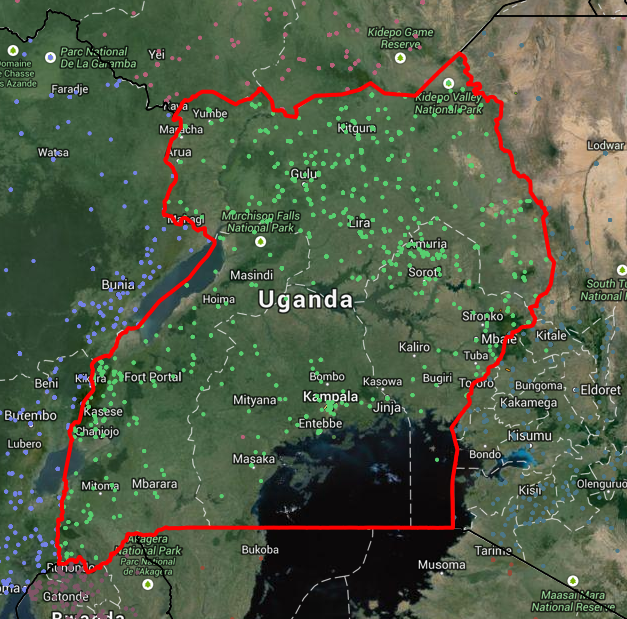
\includegraphics[width=0.6\textwidth]{uganda.png}
  \caption{Civil conflicts in Uganda 1997-2013. [2]}
  \label{fig:map}
\end{figure}

Given a set of simulation data about conflicts (along with historical conflicts), we can now use stochastic optimization techniques
to determine how to distribute aid resources. Our objective function will attempt to model areas that have: (1) a lower risk of violence, (2) a larger 
surrounding population (to serve more refugees), and (3) easy access for aid organizations from neighboring countries. We can then use simulated annealing to optimize over the delivery and placement of food, water, medical resources and shelter to the affected populations.

\section*{Literature Review}

We have reviewed the relevant literature on this problem and found some promising sources. First of
all, a similar effort was made by Sebastian Schutte in his 2010 master's thesis. In it, he used the same ACLED data set in order to predict the occurence of violent conflicts in several African nations. While helpful for us as background information, his focus was on the political science aspect. It seems that he used Monte Carlo methods for simulation, but the methods are not described and our sense is that it was probably specified as a problem for \verb+BUGS+'s black box.

Additionally, we found a helpful paper from the Journal of Statistics Education describing this data set and its potential didactic use for class projects. It was helpful in its description of interesting questions that made be answered by using this ACLED data in conjunction with certain other sources.

Finally, we have reviewed the relevant sections of a number of canonical sources for problems such as these including Gelman and Rubin, Gill, and Bishop.


\subsubsection*{References}

\small{
[1] Armed Conflict Location and Event Data Project, \href{http://www.acleddata.com/data/version-4-data-1997-2013/}{http://www.acleddata.com/data/version-4-data-1997-2013/}.

[2] Map of civil conflicts in Uganda. \href{http://worldmap.harvard.edu/africamap/}{http://worldmap.harvard.edu/africamap/}
}

[3] Bayesian Poisson Regression (as part of the Zelig package in R) \href{http://people.iq.harvard.edu/~falimadh/inst/doc/poisson.bayes.pdf}{http://people.iq.harvard.edu/~falimadh/inst/doc/poisson.bayes.pdf}

\end{document}
